\begin{atiTask}[
  title = Levi-Civita in n-Dimensionen
]

Das \textsc{Levi-Civita}-Symbol ist in $n$ Dimensionen definiert als
\[
\epsilon_{i_1i_2\dots i_n}=\begin{cases}
+1\quad \text{wenn}\quad  i_1,i_2\dots,i_n\quad \text{eine gerade Permutation von 1,2,\dots,n bilden}\\
-1 \quad \quad \text{wenn}\quad i_1,i_2\dots,i_n\quad \text{eine ungerade Permutation von 1,2,\dots,n bilden} \\
0 \quad \text{sonst, d.h. wenn mindestens 2 Indices gleich sind}
\end{cases}
\]
\begin{atiSubtasks}
	\item Bestimmen Sie
	\begin{multicols}{4}
		\begin{atiSubequations}
			\item{\epsilon_{1324}}
			\item{\epsilon_{7125634}}
			\item{\epsilon_{67812345}}
			\item{\epsilon_{364152}}
		\end{atiSubequations}
		\end{multicols}
	(Vorsicht: Nicht einfach loslegen wie in 3 Dimensionen, sondern die o.g. Definition verwenden und ggfs. nachlesen was gerade und ungerade Permuation bedeutet.)
	\item Das Levi-Civita-Symbol kann auch in einer Determinantenschreibweise angegeben werden als
	\[
	\epsilon_{i_1\dots i_n}=\operatorname{det}\begin{pmatrix}
	\rule{0,5cm}{0.3pt} & \vec{e}_{i_1} &\rule{0,5cm}{0.3pt} \\
	\rule{0,5cm}{0.3pt} & \vec{e}_{i_2} & \rule{0,5cm}{0.3pt} \\
	\vdots & \vdots & \vdots \\
	\rule{0,5cm}{0.3pt} & \vec{e}_{i_n} &\rule{0,5cm}{0.3pt}
	\end{pmatrix}, \quad n\in \mathbb{N}
	%\left|\right|
	\]
	Machen Sie sich zunächst klar, dass die Relation stimmt. Stellen Sie dann den Term $\epsilon_{i_1\dots i_n}\cdot\epsilon_{j_1\dots j_n}$ als Determinante dar, indem Sie Eigenschaften von Determinanten und die Relation $\vec{e}_i\vec{e}_j=\delta_{ij}$ verwenden.
	%Berechnen Sie damit explizit $\epsilon{ijk}\epsilon_{ilm}$ (Summenkonvention).
	\item Berechnen Sie mit Hilfe der Determinantenschreibweise $\epsilon_{ijkl}\cdot \epsilon_{mnop}$ und summieren Sie anschließend nacheinander über $i=m$, $j=n$, $k=o$ und $l=p$.
	\item Bestimmen Sie nun allgemein $\epsilon_{i_1\dots i_n}\cdot\epsilon_{i_1\dots i_n}$ (Summenkonvention), wobei hier allgemeine Überlegungen wesentlich schneller zum Ziel führen als das Rechnen mit der Determinantenschreibweise (ist aber auch möglich).
%	\item Erweitern Sie Ihr Ergebnis aus (b) %$\epsilon_{ijk}\epsilon{ilm}=\delta_{jk}\delta_{km}-\delta_{jm}\delta_{kl}$
%	auf den vierdimensionalen Fall $\epsilon_{ijkl}\epsilon{imno}$
\end{atiSubtasks}

\end{atiTask}

\begin{atiSolution}
	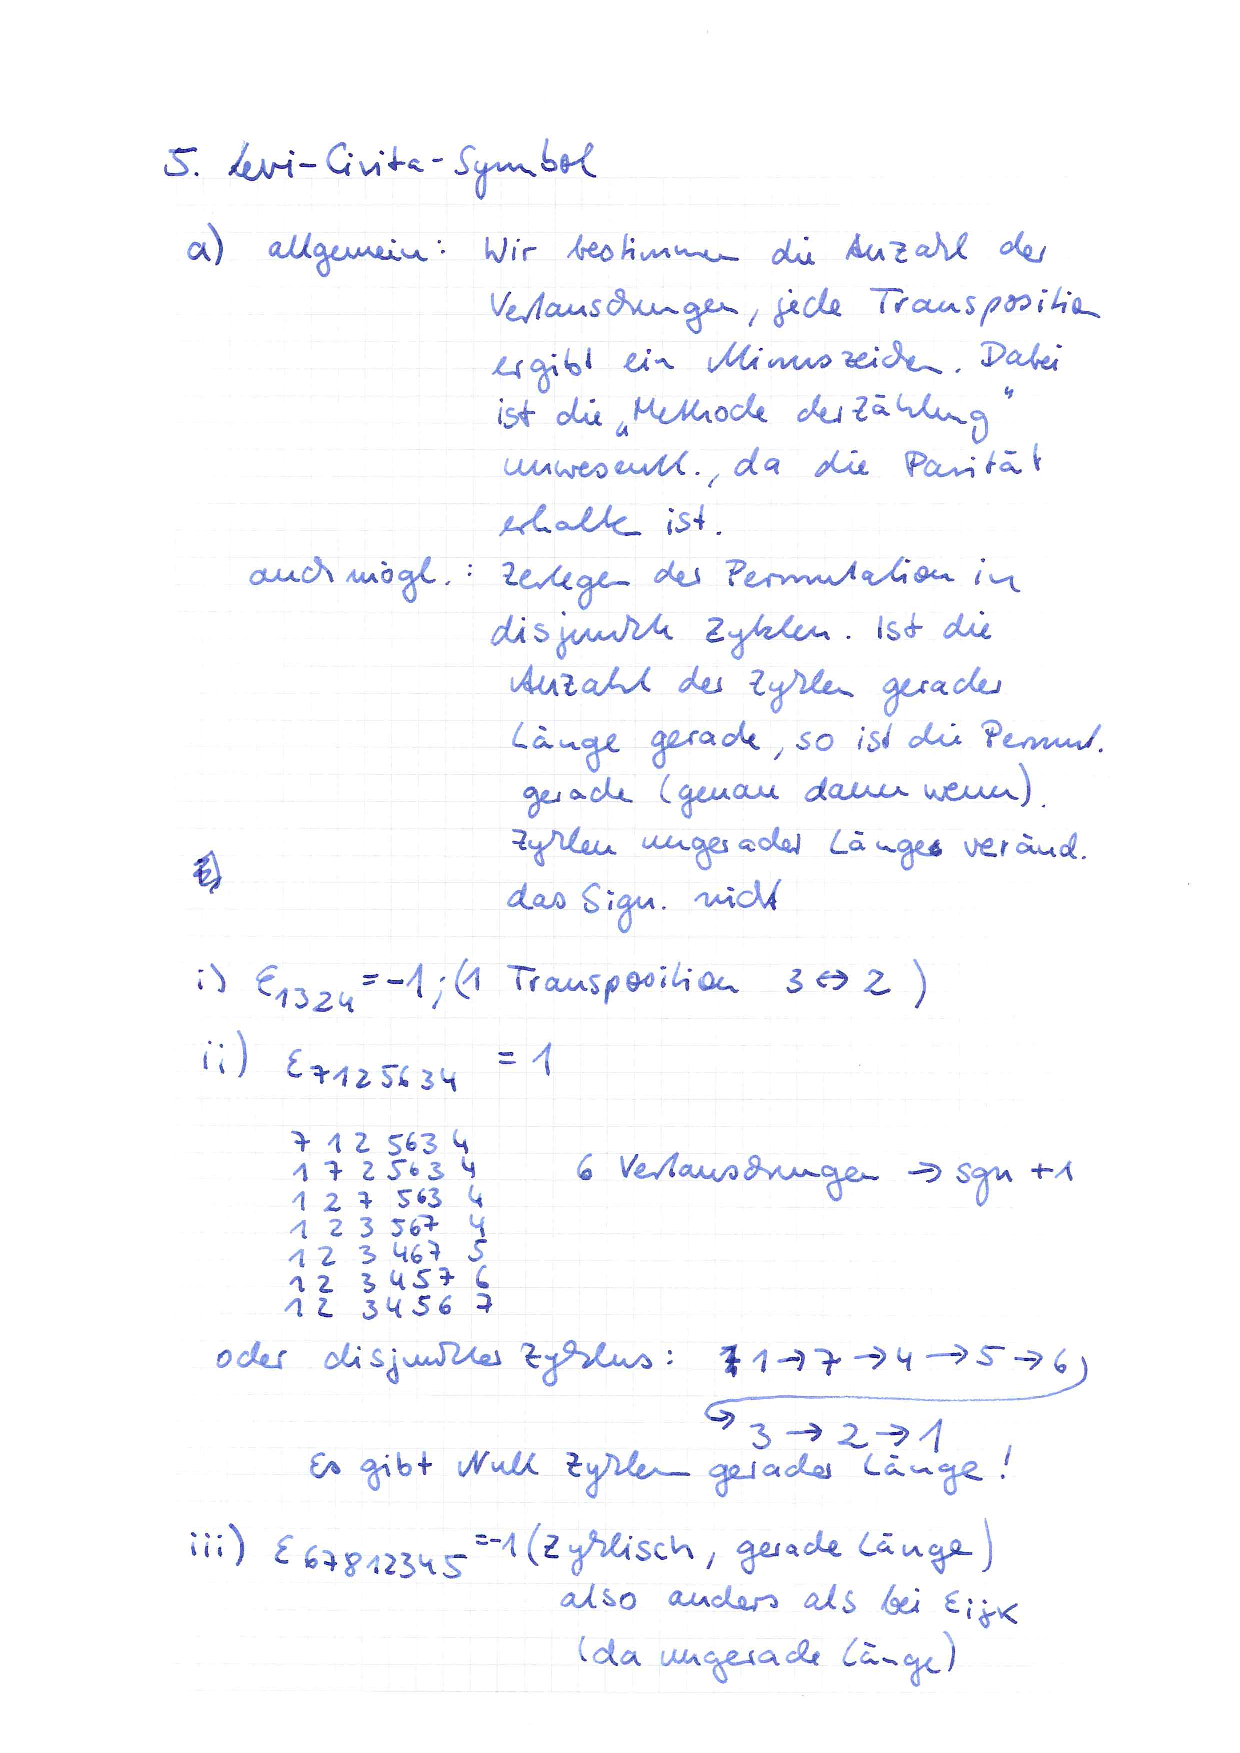
\includepdf[pages=-]{solution-index_v.pdf}
\end{atiSolution}